
\chapter{Experiments, Results and Analysis}
\label{experiments}
\epigraph{Experiment is the sole judge of scientific ``truth''}
{\textit{The Feynman Lectures on Physics, Introduction, Richard Feynman, 1961.}}
The previous chapters have described the models and implementation of the simulation.
This chapter uses the simulation to define experiments to answer questions about CSE, like:
\begin{itemize}
  \item What effect does the probability a user upgrades their system or installs a component have during CSE?
  \item What observations made about the \modelname model in chapter \ref{formal} are observed in the simulation?
  \item Can we alter the criteria employed by the user to reduce change or decrease out-of-dateness?
  \item What are the effects of the new criteria on the evolution of ``real'' systems?
\end{itemize}

Through answering such questions the evolution of Ubuntu systems can be explored,
and the behaviour of CSE described.
The behaviours that are focused on is the amount of change that the system goes through as it evolves,
and how out-of-date it becomes.

%TODO default values for variables

\section{Upgrade and Install Variable Analysis}
How often a user decides to upgrade their system or install a component will effect how the system evolves.
This section attempts to describe how much they differ and how 

\section{Observations}
In chapter \ref{formal} a series of observations about the \modelname model were made.
These observations were:
\begin{itemize}
  \item It is not required for an evolution step to satisfied prior user requests.
  \item Multiple evolution steps may produce a less optimal component system than an equivalent, single evolution step.
  \item Finding a solution to an evolution problem is NP-complete.
\end{itemize}

This section takes these observations and sees whether they are observable during simulation.

\section{Criteria}
Up till this point the criteria used during simulation has reflected the criteria used by apt-get.
This section asks whether altering the criteria used to upgrade a users system if the amount of change can be reduced,
or the system can become less out-of-date.

\subsection{Stable Version}
%%%Here is a real example of this happening
An example of this described situation is show in figures \ref{apachelog} and \ref{apachebug}.

\begin{figure}[htp]
\begin{center}
\begin{alltt}
apache2 (2.2.20-1) unstable; urgency=low

  * New upstream release.
  * Fix some regressions related to Range requests caused by the CVE-2011-3192
    fix. Closes: #639825
\ldots

 -- Stefan Fritsch <sf@debian.org>  Sun, 04 Sep 2011 21:50:22 +0200

apache2 (2.2.19-2) unstable; urgency=high

\ldots

 -- Stefan Fritsch <sf@debian.org>  Mon, 29 Aug 2011 17:08:17 +0200
\end{alltt}
\caption[Apache Changelog]{An extract from the apache changelog located on http://changelogs.ubuntu.com/}
\label{apachelog}
\end{center}
\end{figure}

\begin{figure}[htp]
\begin{center}
\begin{alltt}

Reported by: Takis Issaris <takis.issaris@uhasselt.be>
Date: Tue, 30 Aug 2011 16:09:01 UTC
Severity: important
Found in versions 2.2.9-10+lenny10, 2.2.16-6+squeeze2, apache2/2.2.19-2

\ldots

Package: apache2.2-common
Version: 2.2.9-10+lenny10

Yesterday evenings update broke our Apache server setup,
\ldots
\end{alltt}
\caption[Apache Bug Report]{Extract from the bug report \#639825, filed with Debian}
\label{apachebug}
\end{center}
\end{figure}

A summary of these events are:
\begin{enumerate}
  \item Apache developer Stefan Fritsch released a new version of their server, apache2/2.2.19-2, on 29 Aug 2011
  \item Takis Issaris upgraded to this version which broke his system on 29 Aug 2011
  \item Takis Issaris submits a bug report on 30 Aug 2011, where he and Stefan Fritsch discuss the causes
  \item On 04 Sep 2011 Stefan Fritsch releases a new version 2.2.20-1 that fixes this bug
\end{enumerate}

\subsection{Progressive Upgrade}


\section{Real Evolution}
During the previous experiments how often the user upgrades or installs a component have been assigned values that may not be ``realistic''.
This section presents the final experiments where the variables are assigned values calculated from real user's systems.


%%%%%%%%%%%%%%%%%%%%%%%%%%%%%%%%%%%%
\subsubsection{Extracting Information from the User Submitted Logs}
These variables of update probability and user install probability can be extracted from the user submitted logs from the survey.
Initially, 31 logs where submitted, these logs were filtered to be APT logs, of more than 15 days long.
This resulted in 19 logs of between 23 and 277 days long to be processed.

An extract from one of these logs is shown in figure \ref{aptlog}.
\begin{figure}[htp]
\begin{center}
\begin{alltt}
\ldots
Start-Date: 2010-12-21 11:32:28
Install: libnet-daemon-perl (0.43-1), libhtml-template-perl (2.9-1), libdbi-perl (1.609-1build1), mysql-client-core-5.1 (5.1.41-3ubuntu12.8), libdbd-mysql-perl (4.012-1ubuntu1), mysql-server-5.1 (5.1.41-3ubuntu12.8), mysql-client-5.1 (5.1.41-3ubuntu12.8), libmysqlclient-dev (5.1.41-3ubuntu12.8), libplrpc-perl (0.2020-2), mysql-server-core-5.1 (5.1.41-3ubuntu12.8), mysql-server (5.1.41-3ubuntu12.8), libmysqlclient16-dev (5.1.41-3ubuntu12.8)
Upgrade: mysql-common (5.1.41-3ubuntu12.6, 5.1.41-3ubuntu12.8), libmysqlclient16 (5.1.41-3ubuntu12.6, 5.1.41-3ubuntu12.8)
End-Date: 2010-12-21 11:33:03
\ldots
\end{alltt}
\caption[APT log extract]{An extract of an APT log file}
\label{aptlog}
\end{center}
\end{figure}

These logs mainly describe the changes made to the system by APT, not necessarily what the user requested.
This is because APT may be used through another application, like semantic, to install or update the system.
As the criteria of APT is known, some information about the action the user requested can be inferred.

Given APT will never install or remove a component if the system is updated; 
if a package is upgraded but none are removed or installed then the user probably selected to update.
Also, if a package is installed, then the user requested a single package to be installed.
This second rule is assuming that only one package was selected, and not two at the same time.

Using these rules, each log is processed, and the variables of update probability and install distribution are measured.


\subsubsection{Measuring the Effect}
By calculating the difference in days between each version of all components in the repository, 
over the dates of the simulation how often this situation occurs, where packages are quickly updated, can be measured.
In figure \ref{comeponentversionreleases} a graph is presented measuring the time difference between version releases.
 
\begin{figure}[htp]
\begin{center}
  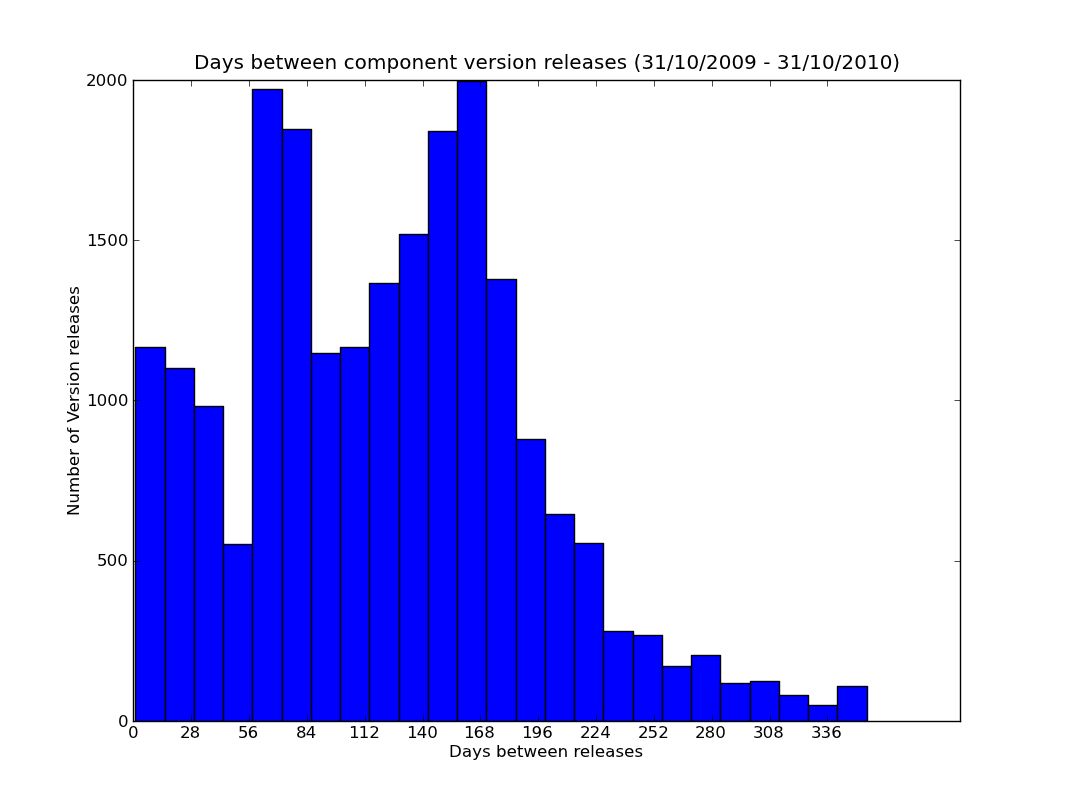
\includegraphics[width=\textwidth]{ubuntusimulationpics/versionreleasedistribution}
  \caption[labelInTOC]{Distribution of the releases of component versions between 31/10/2009 - 31/10/2010}
  \label{comeponentversionreleases}
\end{center}
\end{figure}

There are two points on this graph are noteworthy, firstly there is a large amount of components that release after 3 and 6 months.
Secondly there is a smaller but significant amount of components that have been released less than a month after the previous release.


\section{Summary}
%%%A list of the answers gained from the questions
